\section{Call of Duty}

\begin{figure}[htbp]
\begin{center}
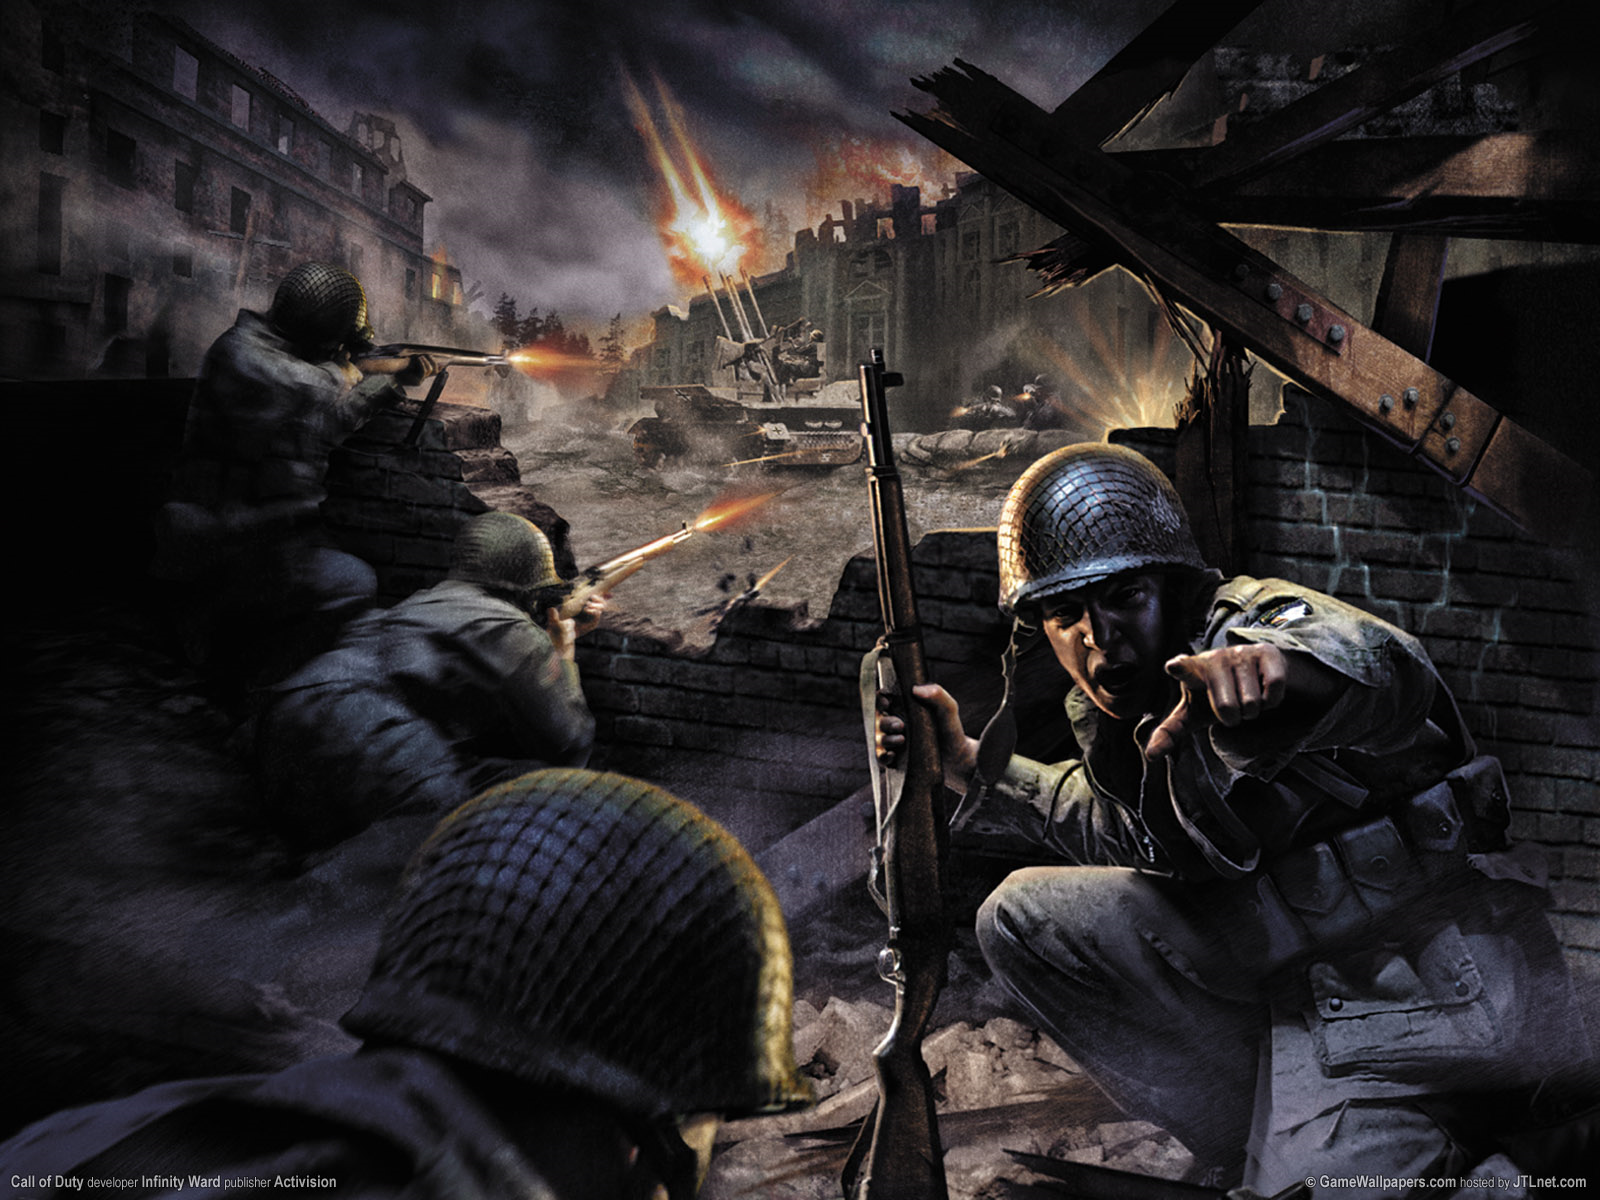
\includegraphics[width=.60\textwidth]{./imagenes/callofduty.png}
\caption{Call of Duty}
\label{Call of Duty}
\end{center}
\end{figure}
Call of Duty \footnote{\url{http://www.callofduty.com/}} es una serie de videojuegos en primera persona (FPS), de estilo bélico, creada por Ben Chichoski, desarrollada principal e inicialmente por Infinity Ward, y distribuida por Activision.
La serie inicialmente se ambientaba en la Segunda Guerra Mundial, relatando personajes y combates acaecidos durante dicho conflicto bélico, recreando las batallas más importantes, llevando al jugador por una serie de escenarios de Europa y el Norte de África, y siempre en la piel de un soldado inglés, estadounidense o soviético; y en menores ocasiones, francés o canadiense.


\subsubsection{¿Por qué es uno de mis juegos favoritos?}
\begin{itemize}
\item Este es un juego que requiere de comunicación para poder lograr el objetivo y poder ganar.  Es uno de los mejores juegos de guerra que hay basados en las guerras mundiales. El juego tiene una gran selección de misiones para elegir, esto quiere decir que cada partida es diferente.
\end{itemize}